\documentclass{article}

\usepackage{mathtools} 
\usepackage{float}
\usepackage{array}
\usepackage{blindtext}
\usepackage{pgfplots}
\usepackage{graphicx}
\usepackage{hyperref}
\usepackage{tikz}
\usepackage{pgfplots}
\usepackage{mathtools, nccmath}
\usepackage{amsmath}
\usepackage{mleftright}
\usepackage{array}

\newenvironment{conditions}
  {\par\vspace{\abovedisplayskip}\noindent\begin{tabular}{>{$}l<{$} @{${}={}$} l}}
  {\end{tabular}\par\vspace{\belowdisplayskip}}

\DeclarePairedDelimiter{\nint}\lfloor\rceil

\newcommand{\lnb}[1]{%
  \ln\mleft(#1\mright)%
}

\pgfplotsset{compat=1.9}

\author{Adrian-Valentin Panaintescu}
\title{Benchmark\\Hill Climbing and Simulated Annealing\\exploring the minimum}
\begin{document}
\maketitle
\begin{abstract}
    Heuristic search refers to a search strategy that attempts to optimize the solution by iteratively improving the solution based on a given heuristic function or a cost measure. A heuristic search method does not always guarantee to find the optimal solution, but may instead find an acceptable solution within a reasonable amount of time and memory space. The most common methods includes hill climbing methods, the best-first search, the A* algorithm, simulated-annealing, and genetic algorithms.
\end{abstract}
\section{Introduction}
    In this article we will describe how these algorithms: Hill Climbing best or first improvement and Simulated Annealing  handle the problem of finding the minimum. The tests are perform using 4 specific mathematical functions:
    \begin{itemize}
        \item De Jong 1 function
        \item Schwefel's function
        \item Rastrigin's function
        \item Michalewicz's function
    \end{itemize}
    Testing for each function all three methods and varying with dimensions: 5, 10, 30.
    Also in the experiment we took into account the accuracy of the numbers and the size of its representation. 
\section{Motivation}
    In this experiment we will analyze how one method is better than another and in what circumstances. And to what extent it influences various parameters such as: \textit{dimension}, \textit{method} or \textit{precizion} result and computation time.
\section{Methods}
    As a mention, the start point is generating into a binary representation by generating \textit{c} $\cdot$ \textit{n bits}. That \textit{c} reprezent minimul of bits used to reprezent o value and is computed in the begining by:
    \begin{equation}
        f(a,b,p) = \nint{\frac{ \lnb{ 10^p \cdot (b - a) }}{\lnb{2}}  }
    \end{equation}
    where:
    \begin{conditions}
        a   &  lower range limit of the domain\\
        b   &  upper range limit of the domain\\
        p   &  precision
    \end{conditions}
    A neighbor is recognized that the difference by binary representation is only a bit.
\subsection{Hill Climbing First Improvement}
    In Hill Climbing technique, starting at the base of a hill, we walk upwards until we reach the top of the hill. In other words, we start with initial state and we keep improving the solution until its optimal. The improvement is made when you find an optimal neighbor.
    \newline
    As a mention, we start from a random point and we are looking through his neighbors and we move on to the first neighbor who is better.
\subsection{Hill Climbing Best Improvement}
    Like Hill Climbing First Improvement, a gradient search is made only that it differs in the fact that all the neighbors are evaluated and the best is our jump.
\subsection{Simulated Annealing}
    It is also a gradient search, only that the neighbors consider themselves a little closer step by step, so that approaching the optimal solution it will converge in the optimal.
\section{Experimental}
    During the experiment each parameter configuration was run 30 times and taken in the minimum, minimum horse but especially the average together with the standard deviation.\\
    The precision was 5 to maintain uniformity and facilitate comparison.\\
    Hill Climbing has an 10000 internal iterations and Simulated Annealing run with start with temperature \textit{T = 200} and accepted temperature \textit{T > 0.00001} and the function for actualization:
    $$f(T) = T \cdot s , s = 0.95 $$

\subsection{Functions}
    Using the following functions, we can argue that the search space is one that does not allow a greedy approach. These functions are characterized by the fact that they have several local optimal and plateau.

    \begin{figure}[H]
        \centering
        \begin{minipage}{.5\textwidth}
            \begin{figure}[H]
                \centering
                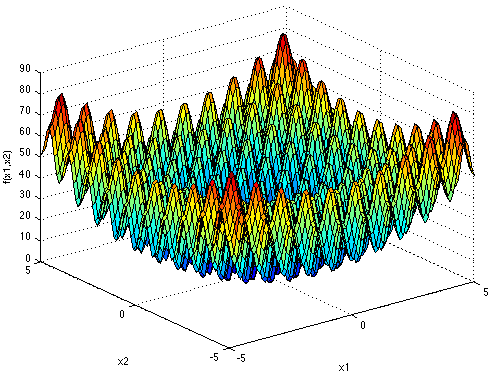
\includegraphics[width=0.9\textwidth,height=\textheight,keepaspectratio]{fig_rastrigin}
                \caption{Rastrigin's Function}
            \end{figure}
        \end{minipage}%
        \begin{minipage}{.5\textwidth}
          \centering
            \begin{figure}[H]
                \centering
                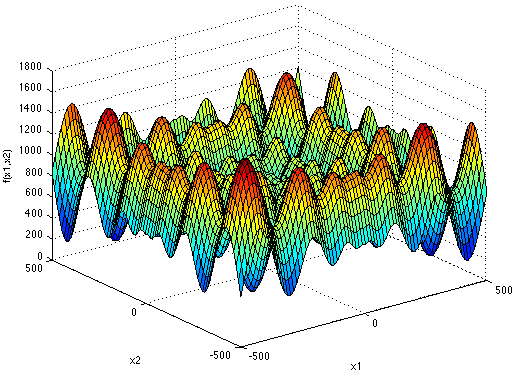
\includegraphics[width=0.9\textwidth,height=\textheight,keepaspectratio]{fig_schwef}
                \caption{Schwefel's Function}
            \end{figure}
        \end{minipage}
        \begin{minipage}{.5\textwidth}
            \begin{figure}[H]
                \centering
                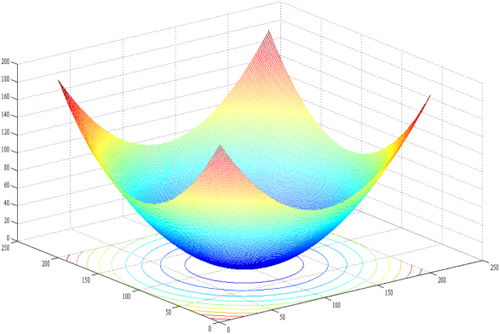
\includegraphics[width=0.9\textwidth,height=\textheight,keepaspectratio]{fig_jong}
                \caption{De Jong 1 Function}
            \end{figure}
        \end{minipage}%
        \begin{minipage}{.5\textwidth}
          \centering
            \begin{figure}[H]
                \centering
                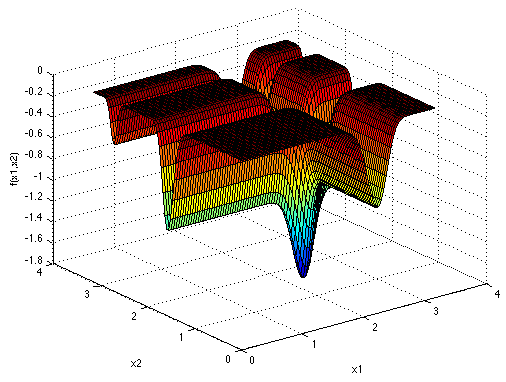
\includegraphics[width=0.9\textwidth,height=\textheight,keepaspectratio]{fig_michal}
                \caption{Michalewicz's Function}
            \end{figure}
        \end{minipage}
    \end{figure}


\subsubsection{De Jong 1}
    $$ f(x) = \sum_{i=1}^n x_i^2, x_i \in \left[ -5.12 , 5.15 \right] $$

\subsubsection{Schwefel's}
    $$ f(x) = \sum_{i=1}^n -x_i \cdot \sqrt{ \left\lvert x_i\right\rvert }, x_i \in \left[ -500 , 500 \right] $$

\subsubsection{Rastrigin's}
    $$ f(x) = A \cdot n + \sum_{i=1}^n x_i^2 - 10 \cdot cos(2 \cdot \pi \cdot x_i) , x_i \in \left[ -5.12 , 5.12 \right] , A = 10 $$

\subsubsection{Michalewicz's}
    $$ f(x) = - \sum_{i = 1}^{n} \sin(x_i) \cdot \left[ \sin( \frac{i \cdot x_i^2}{\pi} ) \right] ^ {2 \cdot m }, x_i \in \left[ 0 , \pi \right] , m = 10  $$

\section{Results}
    \subsection{De Jong 1}
        \begin{figure}[H]
            \centering
            \begin{tabular}{|l|c|c|c|c|c|r|}
                \hline Algorithm & Dim & Mean & Min & Max & Deviation & Time (s) \\
                \hline hc-first & 10 & 0 & 9.76682e-07 & 9.76682e-07 & 8.47033e-22 & 2.08212 \\
                \hline hc-best & 10 & 0 & 2.51984e-05 & 0.000133805 & 2.30341e-05 & 0.812047 \\
                \hline sa & 10 & 0 & 9.76682e-07 & 9.76682e-07 & 8.47033e-22 & 2.04219 \\
                \hline hc-first & 15 & 0 & 1.46502e-06 & 1.46502e-06 & 6.35275e-22 & 3.8621 \\
                \hline hc-best & 15 & 0.00014 & 4.91271e-05 & 0.0016712 & 0.000103252 & 0.705516 \\
                \hline sa & 15 & 0 & 1.46502e-06 & 1.46502e-06 & 6.35275e-22 & 3.95299 \\
                \hline hc-first & 30 & 0 & 2.93004e-06 & 2.93004e-06 & 1.27055e-21 & 0.14188 \\
                \hline hc-best & 30 & 0.00019 & 8.10646e-05 & 0.000568624 & 5.19716e-05 & 0.915175 \\
                \hline sa & 30 & 0 & 2.93004e-06 & 2.93004e-06 & 1.27055e-21 & 8.16611 \\\hline
            \end{tabular}
            \caption{De Jong 1 results table}
        \end{figure}


    \subsection{Schwefel's}
        \begin{figure}[H]
            \centering
            \begin{tabular}{|l|c|c|c|c|c|r|}
                \hline Algorithm & Dim & Mean & Min & Max & Deviation & Time (s) \\
                \hline hc-first & 10 & -3073.32 & -3684.07 & -2624.63 & 193.153 & 2.63315 \\
                \hline hc-best & 10 & -3959.01 & -4189.83 & -3637.51 & 122.819 & 0.691972 \\
                \hline sa & 10 & -3319.24 & -3680.93 & -2730.96 & 221.817 & 2.6178 \\
                \hline hc-first & 15 & -4679.9 & -5291.33 & -3963.48 & 243.603 & 4.70815 \\
                \hline hc-best & 15 & -6027.99 & -6284.12 & -5654.59 & 118.773 & 0.709938 \\
                \hline sa & 15 & -4980.69 & -5510.63 & -4239.05 & 288.24 & 4.67842 \\
                \hline hc-first & 30 & -9342.27 & -9988.14 & -8395.22 & 294.608 & 14.0914 \\
                \hline hc-best & 30 & -11937.5 & -12347.7 & -11407.5 & 175.155 & 1.00358 \\
                \hline sa & 30 & -9888.68 & -10835.3 & -8710.03 & 419.934 & 14.3921 \\
                \hline
            \end{tabular}
            \caption{Schwefel's results table}
        \end{figure}

        \subsection{Rastrigin's}
        \begin{figure}[H]
            \centering
            \begin{tabular}{|l|c|c|c|c|c|r|}
                \hline Algorithm & Dim & Mean & Min & Max & Deviation & Time (s) \\
                \hline hc-first & 10 & 23.8912 & 9.95389 & 40.9455 & 7.12647 & 1.6802 \\
                \hline hc-best & 10 & 13.2314 & 2.99668 & 26.3303 & 6.20286 & 0.584127 \\
                \hline sa & 10 & 20.7069 & 6.95289 & 38.183 & 5.5531 & 1.7013 \\
                \hline hc-first & 15 & 36.9367 & 18.8341 & 49.994 & 7.28582 & 3.00671 \\
                \hline hc-best & 15 & 15.7768 & 6.4644 & 27.418 & 4.98917 & 0.65536 \\
                \hline sa & 15 & 29.3345 & 15.6853 & 48.5941 & 7.20882 & 3.08207 \\
                \hline hc-first & 30 & 73.2062 & 40.4491 & 112.753 & 11.5703 & 8.68145 \\
                \hline hc-best & 30 & 35.0751 & 21.6035 & 54.4033 & 7.20532 & 0.899367 \\
                \hline sa & 30 & 56.7813 & 38.6183 & 75.9252 & 7.05237 & 8.7485 \\
                \hline
            \end{tabular}
            \caption{Rastrigin's results table}
        \end{figure}

        \subsection{Michalewicz's}
        \begin{figure}[H]
            \centering
            \begin{tabular}{|l|c|c|c|c|c|r|}
                \hline Algorithm & Dim & Mean & Min & Max & Deviation & Time (s) \\
                \hline hc-first & 10 & -7.3794 & -8.82491 & -4.40354 & 0.744486 & 2.46225 \\
                \hline hc-best & 10 & -9.21779 & -9.88988 & --8.71383 & 0.284067 & 0.869014 \\
                \hline sa & 10 & -8.10464 & -9.21586 & -6.86494 & 0.598839 & 2.4336 \\
                \hline hc-first & 15 & -11.5333 & -13.6796 & -9.25147 & 0.920931 & 4.85392 \\
                \hline hc-best & 15 & -14.0174 & -14.648 & -13.0156 & 0.348111 & 1.08516 \\
                \hline hc-first & 30 & -22.1946 & -24.4272 & -18.7593 & 0.921606 & 16.4472 \\
                \hline hc-best & 30 & -27.8643 & -29.0349 & -25.9075 & 0.523017 & 1.72776 \\
                \hline sa & 30 & -23.6245 & -27.053 & -20.2618 & 1.36884 & 16.7719 \\
                \hline
            \end{tabular}
            \caption{Michalewicz's results table}
        \end{figure}

\subsection{Obeservation}
    It is clear that the computation time has increased with increasing size but what you could see is that this increase is not more pronounced for Simulated Annealing. \newline
    We can see that the number of dimensions plays a very important role in the purpose the better the number of variables of the function, the weaker the result will be, which does not detract from the the global minimum we want to approach.\newline
    As far as the result and the size are concerned, something like would have a relation: $$ r = dim * C $$ 
\section{Conclusions}
    One method is better than another. I believe that not every method can be classified as the best. It simply depends on the context and we as humans must use our reasoning to decide what and when is best in context with the problem. \newline
    In the future I could run the experiment using some characteristics being variable, such as computing machinery or different precision.

\begin{thebibliography}{9}

    \bibitem{fct_1}
        Wiley, De Jong 1's function figure \\
        \url{https://onlinelibrary.wiley.com/cms/asset/ab373f57-0fc8-41a3-99bb-a85c8931e035/cplx21560-fig-0012-m.png}\\
    \bibitem{fct_2}
        Sfu, Schwefel’s function figure \\
        \url{https://www.sfu.ca/~ssurjano/schwef.html}\\
    \bibitem{fct_3}
        Sfu, Rastrigin’s function figure \\
        \url{https://www.sfu.ca/~ssurjano/rastr.html}\\
    \bibitem{fct_4}
        Sfu, Michalewicz's function figure \\
        \url{https://www.sfu.ca/~ssurjano/michal.html}

    \bibitem{tex_tuturial}
        Stackexchange.com \\ pgfplot: 3d function plot \\
        \url{https://tex.stackexchange.com/questions/194018/pgfplot-3d-function-plot}\\
    \bibitem{pgfplots_man}
        Manual for Package pgfplots \\
        \url{http://pgfplots.sourceforge.net/pgfplots.pdf}
    \bibitem{sa_tuturial}
        Wikipedia \\ Simulated Annealing \\
        \url{https://en.wikipedia.org/wiki/Simulated_annealing}
    \bibitem{sa2_tuturial}
        Simulated Annealing on Sciencedirect \\
        \url{https://www.sciencedirect.com/topics/materials-science/simulated-annealing}
    \bibitem{heuristic_tuturial}
        Springer \\ Heuristic Search \\
        \url{https://link.springer.com/referenceworkentry/10.1007%2F978-1-4419-9863-7_875}
    \bibitem{sample_hc_java}
        Baeldung \\ Example of Hill Climbing Algorithm in Java \\
        \url{https://www.baeldung.com/java-hill-climbing-algorithm}
    \bibitem{yt_hc}
        Youtube \\ Hill Climbing Algorithm \\
        \url{https://www.youtube.com/watch?v=oSdPmxRCWws}
    \bibitem{profs_ga}
        profs.info.uaic.ro \\ Teaching: Genetic Algorithms
        \url{https://profs.info.uaic.ro/ eugennc/teaching/ga/}
    \bibitem{tex_notation_ceil}
        Stackexchange.com \\ Rounding to nearest integer symbol in Latex \\
        \url{https://tex.stackexchange.com/questions/433101/rounding-to-nearest-integer-symbol-in-latex}
    \bibitem{tex_side_by_side}
        Stackexchange.com \\ LaTeX figures side by side \\
        \url{https://tex.stackexchange.com/questions/37581/latex-figures-side-by-side}
    \bibitem{tex_ln_view}
        Stackexchange.com \\ No natural log parentheses when typesetting\\
        \url{https://tex.stackexchange.com/questions/314609/no-natural-log-parentheses-when-typesetting}
    \bibitem{tex_comment_equation}
        Stackexchange.com \\ How to write a perfect equation parameters description\\
        \url{https://tex.stackexchange.com/questions/95838/how-to-write-a-perfect-equation-parameters-description}

\end{thebibliography}

\end{document}
